\section{Tecnología Existente}

\par \noindent
En los últimos años todos los avances en aspectos de tecnología se ha sido gracias al Internet. La implementación del Internet a los celulares dio paso a un mejora en los componentes utilizados para la fabricación de los mismos y nuevas características. El nacimiento de nuevos sistemas operativos para celulares como iOS y Android, junto con sus aplicaciones transformando lo que antes era solo un dispositivo para hacer llamadas, a una computadora del tamaño de nuestras manos. En el campo de la electrónica los precios de los componentes han ido decayendo. Nace entonces la plataforma educativa Arduino y con ella una vasta documentación para el desarrollo de proyecto como estaciones de temperatura, automatización en el hogar y mucho mas. Según lo mencionado es necesario un análisis mas en detalle de todas las tecnologías que serán utilizadas para el desarrollo de nuestro proyecto.

\subsection{Smartphone}

\par 
El teléfono inteligente (smartphone en inglés) es un tipo de ordenador de bolsillo que combina los elementos de una tablet con los de un teléfono celular. Sobre una plataforma informática móvil, con mayor capacidad de almacenar datos y realizar actividades, semejante a la de una minicomputadora, y con una mayor conectividad que un teléfono móvil convencional. El término inteligente, que se utiliza con fines comerciales, hace referencia a la capacidad de usarse como un computador de bolsillo, y llega incluso a reemplazar a una computadora personal en algunos casos\cite{smartphone}.
	
\par \noindent
Generalmente, los teléfonos con pantallas táctiles son los llamados teléfonos inteligentes, pero el soporte completo al correo electrónico parece ser una característica indispensable encontrada en todos los modelos existentes y anunciados desde 2007\cite{smartphone}.
		
\par \noindent
Entre otros rasgos comunes está la función multitarea, el acceso a Internet vía Wifi o redes 2G, 3G o 4G, función multimedia (cámara y reproductor de videos/mp3), a los programas de agenda, administración de contactos, acelerómetros, GPS y algunos programas de navegación, así como ocasionalmente la habilidad de y leer documentos de negocios en variedad de formatos como PDF y Microsoft Office\cite{smartphone}.

\par \noindent
Los sistemas operativos móviles más frecuentes utilizados por los teléfonos inteligentes son Android (de Google), iOS (de Apple) y Windows 10 (de Microsoft)\cite{smartphone}.

\begin{figure}[H]
	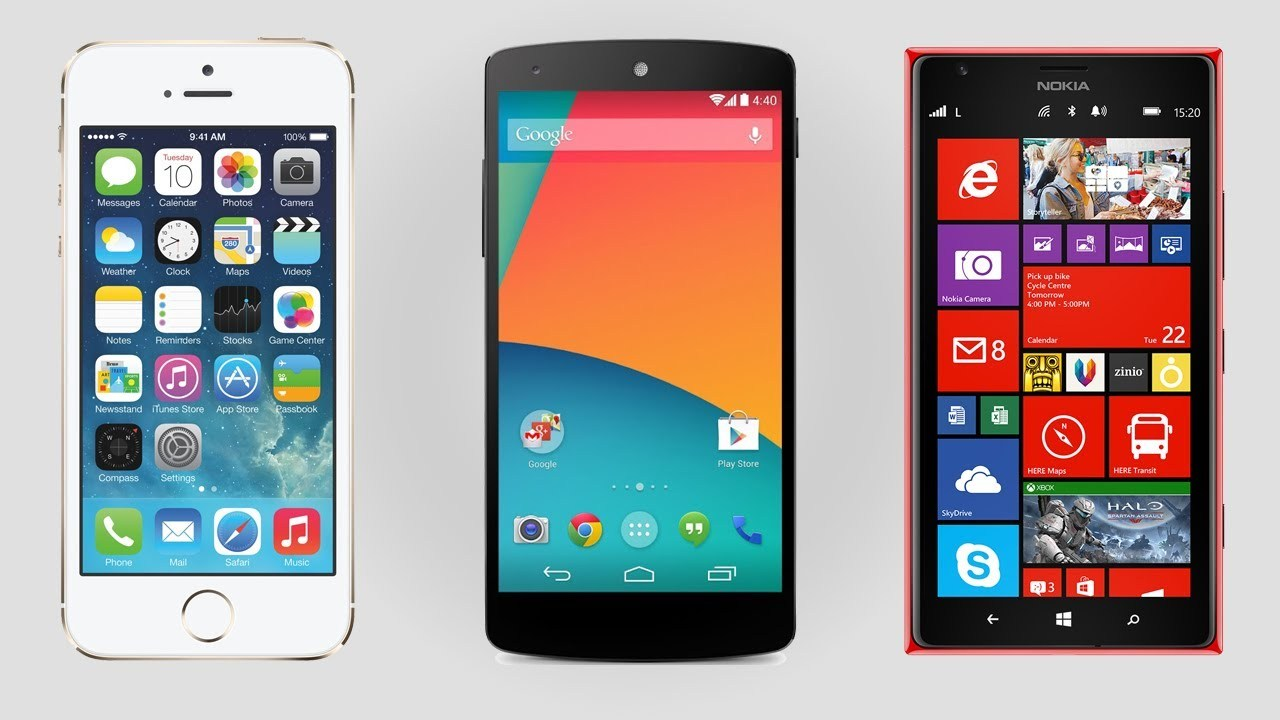
\includegraphics[width=\textwidth]{smartphone1.jpg}
	\caption{Smartphones con los Sistemas Operativos Móviles Mas Populares}
\end{figure}

\par \noindent
En nuestro trabajo utilizaremos exclusivamente para desarrollar el sistema operativo movil Android, debido a su popularidad en el mercado y su vasta documentación para desarrollar aplicaciones.

\subsection{Android}

\par
Android es un sistema operativo basado en el núcleo Linux. Fue diseñado principalmente para dispositivos móviles con pantalla táctil, como teléfonos inteligentes, tablets o tabléfonos; y también para relojes inteligentes, televisores y automóviles. Inicialmente fue desarrollado por Android Inc. la cual fue fundado en 2003 por Andy Rubin, Rich Miner, Nick Sears y Chris White con el objetivo de desarrollar \textquotedblleft dispositivos móviles que están al corriente de la ubicación y preferencias del usuario \textquotedblright\cite{android-wiki}. En un principio la intención era desarrollar un sistema operativo avanzado para cámaras digitales, pero más tarde se cambió el foco al determinar que el mercado de las cámaras digitales no era lo suficientemente grande. Se redirigirían los esfuerzos a crear un sistema que pudiera competir con Symbian y Windows Mobile\cite{android-xataka}. La versión básica de Android es conocida como Android Open Source Project (AOSP)\cite{android-wiki}. A continuación, una imagen de la evolución del logo de Android. 

\begin{figure}[H]
	
\includegraphics[width=\textwidth]{android1.jpg}
	\caption{Diseño preliminar para el logo de Android (Izquierda) y el logo oficial (Derecha)}
\end{figure}

\par \noindent
A partir del año 2011 Google ha ido actualizando la versión de Android, todos los años. Hoy en día la última versión de Android es \textquotedblleft Android 8.0 Oreo \textquotedblright. Sin embargo, la versión de Android con más dispositivo o smartphones, en uso actualmente, es Android 5.0 Lollipop, la cual será presentada a continuación.

\subsubsection{Android 5.0 Lollipop} 

\par 
Android Lollipop es una versión del sistema operativo para dispositivos móviles Android. Fue dada a conocer el 25 de junio de 2014 durante el Google I/O 2014 como Android L, Google I/O es una conferencia anual presentada por Google en sus oficinas en Mountain View, California.
Los cambios más prominentes en Lollipop incluyen una interfaz de usuario rediseñada construida sobre un diseño de lenguaje responsivo denominado como \textquotedblleft Material design\textquotedblright, así como mejoras en el sistema de notificaciones que permiten que este sea accedido desde la pantalla de bloqueo, y mostrado junto con otras aplicaciones como banners en la parte superior de la pantalla. También se realizaron cambios internos para mejorar y optimizar el rendimiento de consumo de batería en smartphones\cite{lollipop}.

\begin{figure}[H]
	\centering
	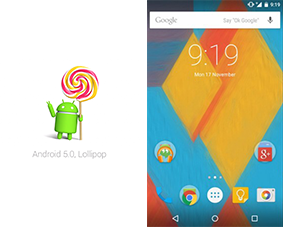
\includegraphics[width=7cm, height=6cm]{android2.png}
	\caption{Logo oficial (Izquierda) e Interfaz móvil (Derecha) de Android 5.0 Lollipop}
\end{figure}

\par \noindent
Ahora veremos las tecnologías que se aplicaran en el área de la electrónica.

\subsection{Arduino}

\par
Arduino es una plataforma de electrónica de código abierto basada en hardware y software fácil de usar. Las placas Arduino pueden leer entradas (luz en un sensor, un dedo en un botón o un mensaje de Twitter) y convertirlo en una salida, activar un motor, encender un LED y publicar algo en línea. Puede decirle a su placa qué hacer enviando un conjunto de instrucciones al microcontrolador en la placa. Para hacerlo, utiliza el lenguaje de programación Arduino (basado en \textquotedblleft Wiring\textquotedblright) y el software Arduino (IDE), basado en \textquotedblleft Processing \textquotedblright\cite{arduino-intro}.

\begin{figure}[H]
	\centering
	
\includegraphics[width=5cm, height=4cm]{arduino1.png}
	\caption{Logo Oficial de Arduino}
\end{figure}

\par \noindent
Con los años, Arduino ha sido el cerebro de miles de proyectos, desde objetos cotidianos hasta complejos instrumentos científicos. Una comunidad mundial de fabricantes (estudiantes, aficionados, artistas, programadores y profesionales) se ha reunido en torno a esta plataforma de código abierto, sus contribuciones se han añadido a una increíble cantidad de conocimiento accesible que puede ser de gran ayuda para principiantes y expertos por igual\cite{arduino-intro}.

\subsection{Sensores en General}

\par
Un sensor es un dispositivo capaz de detectar magnitudes físicas o químicas, llamadas variables de instrumentación, y transformarlas en variables eléctricas.

\begin{itemize}
	\item Las variables de instrumentación pueden ser por ejemplo: temperatura, intensidad lumínica, distancia, aceleración, inclinación, desplazamiento, presión, fuerza, torsión, humedad, movimiento, pH, etc.
	
	\item Una variable eléctrica puede ser una resistencia eléctrica (como en una RTD), una capacidad eléctrica (como en un sensor de humedad o un sensor capacitivo), una tensión eléctrica (como en un termopar), una corriente eléctrica (como en un fototransistor), etc.
\end{itemize}

\par \noindent
Los sensores se pueden clasificar en función de los datos de salida en: digitales y analógicos\cite{sensores-arduino}.

\subsubsection{Características de los Sensores \cite{sensores-wiki}}

\begin{itemize}
	
	\item Rango de medida: dominio en la magnitud medida en el que puede aplicarse el sensor.
	
	\item Precisión: es el error de medida máximo esperado.
	
	\item Offset o desviación de cero:  valor de la variable de salida cuando la variable de entrada es nula. Si el rango de medida no llega a valores nulos de la variable de entrada, habitualmente se establece otro punto de referencia para definir el offset.
	
	\item Linealidad o correlación lineal.
	
	\item Sensibilidad de un sensor: suponiendo que es de entrada a salida y la variación de la magnitud de entrada.
	
	\item Resolución: mínima variación de la magnitud de entrada que puede detectarse a la salida.
	
	\item Rapidez de respuesta: puede ser un tiempo fijo o depender de cuánto varíe la magnitud a medir. Depende de la capacidad del sistema para seguir las variaciones de la magnitud de entrada.
	
	\item Derivas: son otras magnitudes, aparte de la medida como magnitud de entrada, que influyen en la variable de salida. Por ejemplo, pueden ser condiciones ambientales, como la humedad, la temperatura u otras como el envejecimiento (oxidación, desgaste, etc.) del sensor.
	
	\item Repetitividad: error esperado al repetir varias veces la misma medida.
	
\end{itemize}

\par \noindent
Debido a que solamente la magnitud física que nos interesa para nuestro proyecto es la temperatura. Tomamos encuenta los posibles candidatos para utilizar como sensor de temperatura en el prototipo.

\clearpage

\subsubsection{Sensores de Temperatura}	

\paragraph{DS18B20}
El termómetro digital DS18B20 proporciona de 9 bits a 12 bits.
Mediciones de temperatura en grados celsius y tiene una función de alarma no volátil programable por el usuario. El DS18B20 se comunica a través de un Bus de 1 cable que por definición requiere solo una línea de datos (y tierra) para la comunicación con un microprocesador central. Además, el DS18B20 puede obtener potencia directamente desde la línea de datos, eliminando la necesidad de una fuente de alimentación externa\cite{ds18b20}.

\begin{figure}[H]
	\centering
	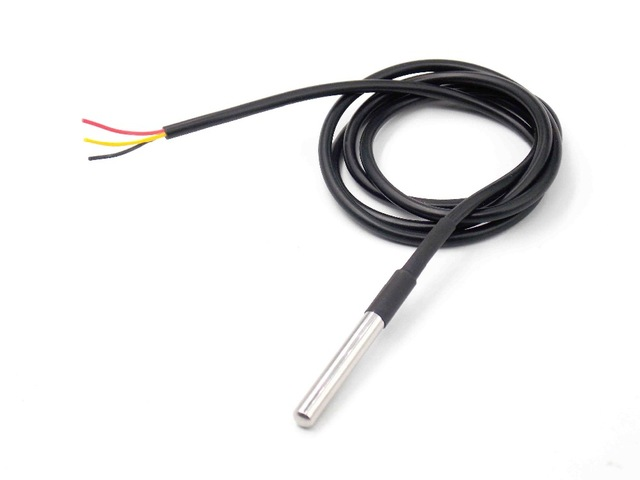
\includegraphics[width=0.5\textwidth]{sensores1.jpg}
	\caption{Sensor DS18B20 estilo sonda}
\end{figure}

\par \noindent
Mide las temperaturas de -55 ° C a 125 ° C, ± 0.5 ° C de  precisión entre -10 ° C a + 85 ° C y resolución programable de 9 a 12 bits.

\par \noindent
Las aplicaciones que pueden beneficiarse de esta característica incluyen
Controles ambientales, monitoreo de temperatura
sistemas dentro de edificios, equipos o maquinaria, y
sistemas de monitoreo y control de procesos\cite{ds18b20}. 


\paragraph{DHT11}
El sensor digital de temperatura y humedad DHT11 es un sensor compuesto que contiene una
señal digital de salida de la temperatura y la humedad. Aplicación de módulos digitales dedicados
tecnología de recolección y la tecnología de detección de temperatura y humedad, para asegurar que
el producto tiene una alta fiabilidad y una excelente estabilidad a largo plazo. El sensor incluye un sentido resistivo
de componentes húmedos y dispositivos de medición de temperatura NTC, y conectado con un
microcontrolador de alto rendimiento de 8 bits\cite{dht11}.

\begin{figure}[H]
	\centering
	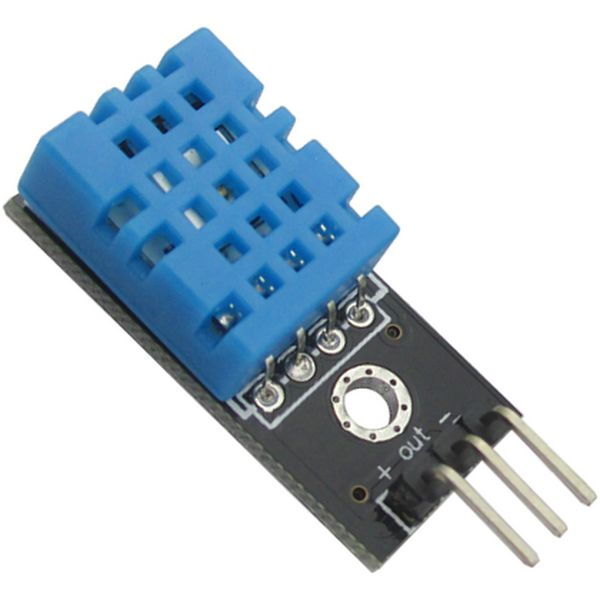
\includegraphics[width=0.25\textwidth]{sensores2.jpg}
	\caption{Sensor DHT11 en placa}
\end{figure}

\par \noindent
Mide temperaturas de 0 ° C a 50 ° C con una precisión de ±2 ° C en 25 ° C y una resoluación no programable de 16 bits.

\par \noindent
Aplicaciones de este sensor son principalmente para mediciones de humedad y temperatura relativa. Donde se require obtener valores en ambas magnitudes y no tanta precisión de una magnitud en particular\cite{dht11}. 

\par \noindent
Los sensores de temperatura y la plataforma de Arduino nos permite crear un prototipo de medición de temperatura; sin embargo, aun no es un termómetro como tal y mucho menos uno que SIGCSA pueda utilizar en campo. Hay que definir el concepto de termómetro para aplicarlo en nuestro prototipo.



\subsection{Termómetros}

\par 
El termómetro es un instrumento de medición de temperatura. Desde su invención ha evolucionado mucho, principalmente a partir del desarrollo de los termómetros electrónicos digitales. La manera como un termómetro determina la temperatura dependera del tipo de termómetro que sea\cite{termometro}. 

\par \noindent
Inicialmente se fabricaron aprovechando el fenómeno de la dilatación, por lo que se prefería el uso de materiales con elevado coeficiente de dilatación, de modo que, al aumentar la temperatura, su estiramiento era fácilmente visible. La sustancia que se utilizaba más frecuentemente en este tipo de termómetros ha sido el mercurio, encerrado en un tubo de vidrio que incorporaba una escala graduada, pero también alcoholes coloreados en termómetros grandes\cite{termometro}.

\begin{figure}[H]
	\centering
	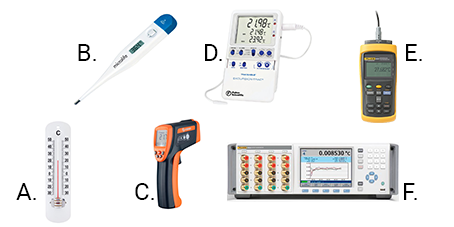
\includegraphics[width=\textwidth]{termometro1.png}
	\caption{Ejemplos de diferentes tipos de termómetros}
\end{figure}

\subsubsection{Escalas de temperatura \cite{termometro}}

\par 
La escala más usada en la mayoría de los países del mundo es la Celsius (\textdegree{}C) en honor a Anders Celsius (1701-1744) que se llamó centígrado hasta 1948. En esta escala, el cero (0 \textdegree{}C) y los cien (100 \textdegree{}C) grados corresponden respectivamente a los puntos de congelación y de ebullición del agua, ambos a la presión de 1 atmósfera.

\par \noindent 
Otras escalas termométricas son:

\begin{itemize}
	
\item Fahrenheit (\textdegree{}F) 

Propuesta por Daniel Gabriel Fahrenheit en la revista Philosophical Transactions (Londres, 33, 78, 1724). El grado Fahrenheit es la unidad de temperatura en el sistema anglosajón de unidades, utilizado principalmente en Estados Unidos.

\item Kelvin (K) o temperatura absoluta: 

Es la escala de temperatura del Sistema Internacional de Unidades. Aunque la magnitud de una unidad Kelvin (K) coincide con un grado Celsius (\textdegree{}C), el cero se ha fijado en el cero absoluto a -273,15 \textdegree{}C y es inalcanzable según el tercer principio de la termodinámica.
\end{itemize}

\subsubsection{Tipos de termómetros \cite{termometro}}

\begin{itemize}
\item Termómetro de mercurio: es un tubo de vidrio sellado que contiene mercurio, cuyo volumen cambia con la temperatura de manera uniforme. Este cambio de volumen se aprecia en una escala graduada. El termómetro de mercurio fue inventado por Gabriel Fahrenheit en el año 1714. Ver figura 2.14 (A)

\item Pirómetros:  termómetros para altas temperaturas, se utilizan en fundiciones, fábricas de vidrio, hornos para cocción de cerámica, etc. Existen varios tipos según su principio de funcionamiento:

\begin{itemize}

\item Pirómetro óptico: se basan en la ley de Wien de distribución de la radiación térmica, según la cual, el color de la radiación varía con la temperatura. El color de la radiación de la superficie a medir se compara con el color emitido por un filamento que se ajusta con un reostato calibrado. Se utilizan para medir temperaturas elevadas, desde 700 °C hasta 3.200 °C, a las cuales se irradia suficiente energía en el espectro visible para permitir la medición óptica. Ver figura 2.14 (B)

\end{itemize}

\item Termómetro de lámina bimetálica: formado por dos láminas de metales de coeficientes de dilatación muy distintos y arrollados dejando el coeficiente más alto en el interior. Se utiliza sobre todo como sensor de temperatura en el termohigrógrafo.

\begin{figure}[H]
\centering
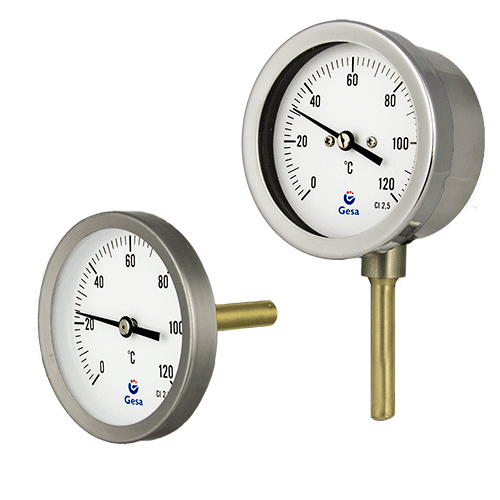
\includegraphics[width=5cm, height=5cm]{termometro2.png}
\caption{Ejemplo de termómetro de lámina bimetálica}
\end{figure}

\item Termómetro de gas: pueden ser a presión constante o a volumen constante. Este tipo de termómetros son muy exactos y generalmente son utilizados para la calibración de otros termómetros.

\begin{figure}[H]
\centering
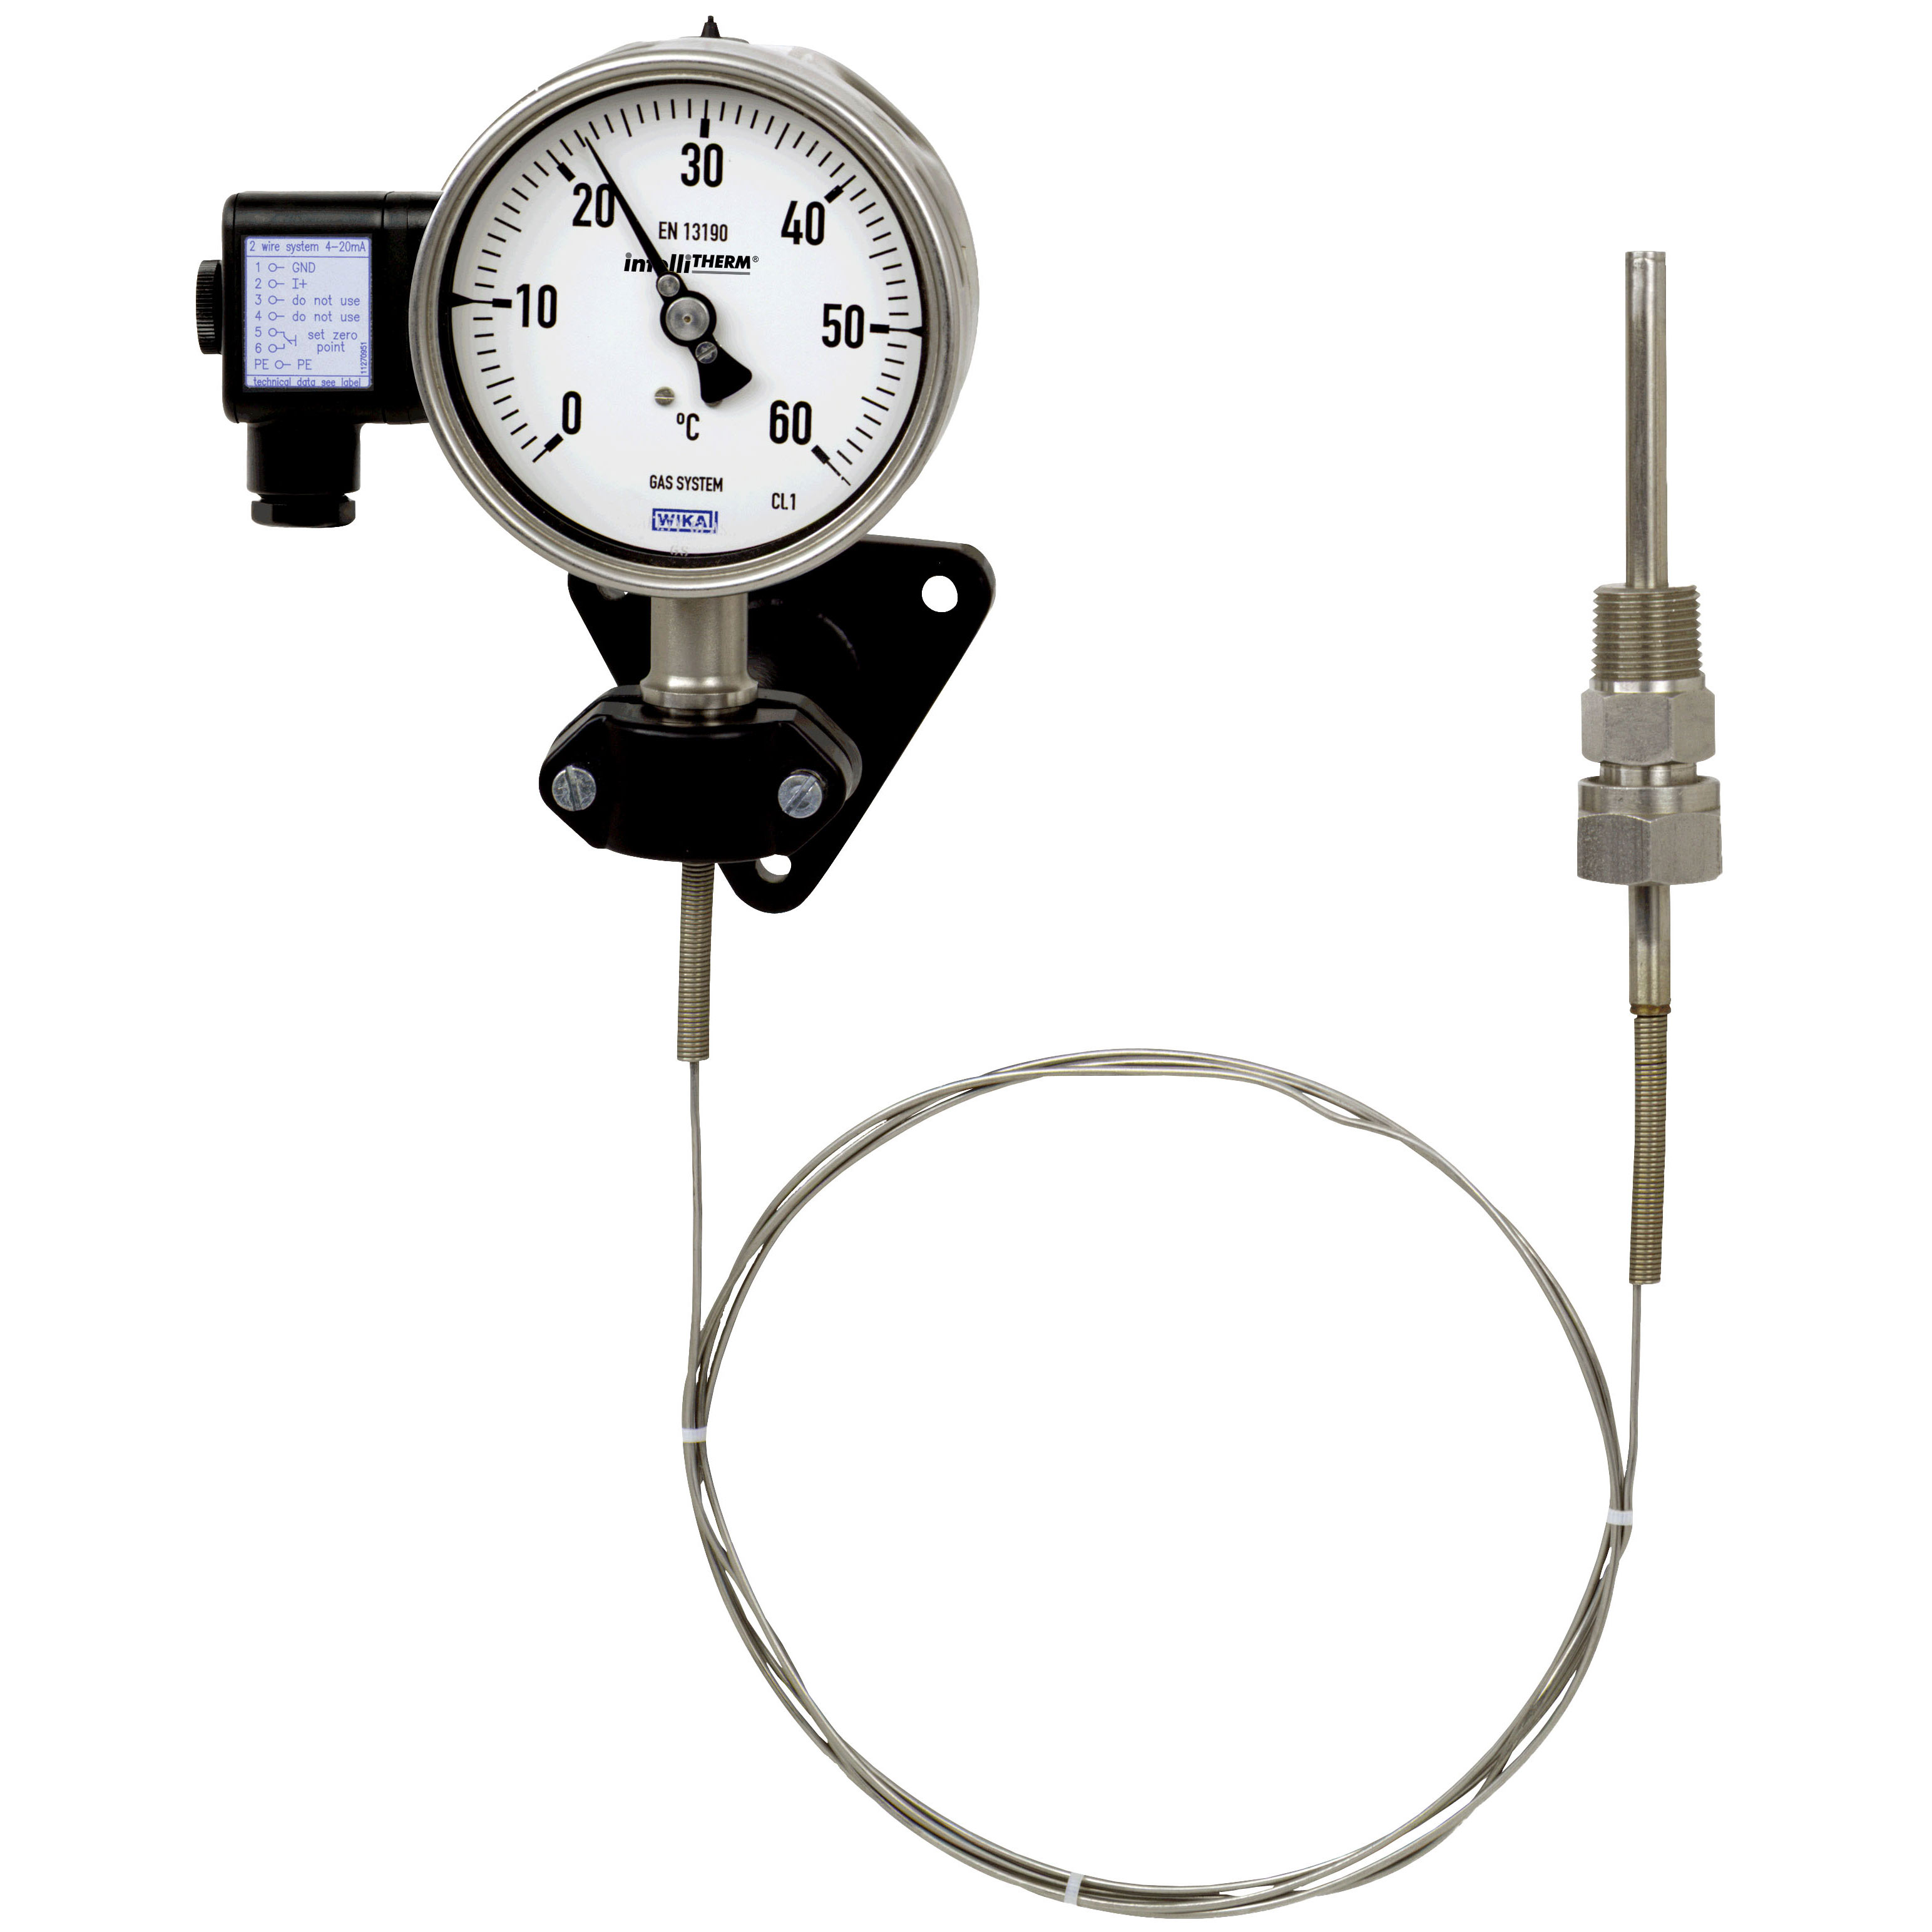
\includegraphics[width=4cm, height=4cm]{termometro3.jpg}
\caption{Ejemplo de termómetro de gas}
\end{figure}

\item Termómetros digitales: son aquellos que, valiéndose de dispositivos transductores, utilizan luego circuitos electrónicos para convertir en números las pequeñas variaciones de tensión obtenidas, mostrando finalmente la temperatura en un visualizador. Una de sus principales ventajas es que por no utilizar mercurio no contaminan el medio ambiente cuando son desechados. Los dispositivos visualizadores pueden ser:

\begin{itemize}

\item Resistencia de platino: consiste en un alambre de algún metal de platino cuya resistencia eléctrica cambia cuando varía la temperatura. Van conectados a un termómetro digital como en la figura 2.14 (D, E y F)

\item Termopar: Tambien conocido comoo termocupla es un dispositivo utilizado para medir temperaturas basado en la fuerza electromotriz que se genera al calentar la soldadura de dos metales distintos. Van conectados a un termómetro digital como en la figura 2.14 (D y E)

\item Termistor:  es un dispositivo que varía su resistencia eléctrica en función de la temperatura. Algunos termómetros hacen uso de circuitos integrados que contienen un termistor, como el LM35. Van conectados a un termómetro digital como en la figura 2.14 (D y E)

\end{itemize}

\item Termómetros clinicos: son los utilizados para medir la temperatura corporal. Los hay tradicionales de mercurio y digitales, teniendo estos últimos algunas ventajas adicionales como su fácil lectura, respuesta rápida, memoria y en algunos modelos alarma vibrante. Ver figura 2.14 (B)

\item Termógrafo: El termógrafo es un termómetro acoplado a un dispositivo capaz de registrar, gráfica o digitalmente, la temperatura medida en forma continua o a intervalos de tiempo determinado. En la figura 2.14 (F) las mediciones van acompañadas de una grafica.
	
\end{itemize}

\par \noindent
Podemos definir que nuestro prototipo sera un termómetro digital, el cual utilizara un termistor en su sensor de temperatura, ver figura 2.12. El ultimo componente de nuestro prototipo es su diseño o armazón donde colocaremos los componentes previamente mencionados. La manera como vamos a ingeniar el armazón sera utilizando la impresión 3D.



\subsection{Impresión 3D}

\par
Es necesario definir el concepto de prototipo porque es el punto de partida para el desarrollo de la tecnología de Prototipado Rapido y consecuentemente, para las impresoras tridimensionales. Podemos definir como prototipo al primer ejemplar que se fabrica de una figura, un invento o elemento físico, y sirve de modelo para fabricar otros iguales.  

\par \noindent
Los prototipos tiene el propósito de probar suposiciones formuladas en busca de una solución a un problema determinado. Ademas se convierten en un diseño enfocado al usuario, donde es necesario un proceso interactivo entre el propio diseñador y el consumidor. Así mismo, todos los prototipos son objetos de desarrollo de bajo costo, pero en muchas ocasiones la necesidad de elaborar varios prototipos o de realizar un prototipo con una estética cuidada, eleva los costes de producción. Por lo tanto, el alto coste de producción de prototipos y tiempo de ejecución de los mismos puede suponer un problema.

\par \noindent
Los sistemas de Prototipado Rápido surgen con la necesidad de solventar estos problemas en el uso de prototipos, se busca por lo tanto, una manera de elaborarlos con un aspecto cuidado y atractivo para el usuario, con un método de fabricación rápido y fácil de modificar, económicos y que pueden ser probados por el consumidor. Por consiguiente, esta herramienta resultará útil y funcional. Rápidamente estos sistemas de construcción aditiva partirán del desarrollo tecnológico de maquinara destinada a uso industrial\cite{impresoras3d-valverde}. 

\begin{figure}[H]
	\centering
	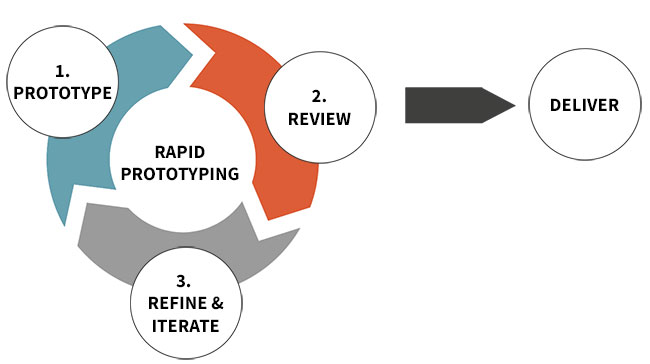
\includegraphics[width=0.5\textwidth]{impresion1.jpg}
	\caption{Ciclo del Prototipado Rapido}
\end{figure}

\par \noindent
El Prototipado Rápido se convierte así, en un proceso utilizado para la fabricación de prototipos, los cuales, como hemos visto, son objetos que no estan diseñados a uso final, sino más bien a modo de prueba de diseño\cite{impresoras3d-valverde}.

\par \noindent
La impresión 3D, también conocida como impresión tridimensional, es un método para
producir objetos tridimensionales con un aparato tecnológico al colocar varias capas
bidimensionales de cierto material una sobre la otra. El proceso es similar a la impresión
bidimensional en la cual se coloca tinta sobre papel, sin embargo, en la impresión
tridimensional se coloca plástico sobre una superficie que nos permite fabricar objetos de tres
dimensiones. Esta tecnología se utiliza principalmente en la producción de prototipos durante
el diseño de algún nuevo producto.

\par \noindent
Durante los últimos años, la tecnología de impresión tridimensional ha avanzado de
manera exponencial. Este tipo de impresoras se han vuelto cada vez más accesibles y por ello
ahora es común encontrarlas en fábricas, industrias, instituciones educativas, instituciones de
investigación e inclusive para uso personal\cite{impresoras3d-monterrey}.

\subsubsection{Técnicas de Impresión 3D}

\par \noindent
Hablaremos de las principales técnicas comerciales de impresión 3D; ya que, la impresión 3D es una tecnología de hace muchos años. No fue hasta a mediados de la década del 2000 que la impresoras 3D comenzaron a bajar sus precios y apuntados a un mercado menos especializado.

\begin{figure}[H]
	\centering
	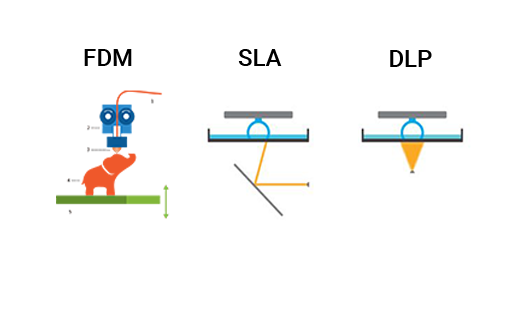
\includegraphics[width=0.8\textwidth]{impresion2.png}
	\caption{Principales Técnicas Comerciales de Impresion 3D}
\end{figure}

\paragraph{FDM (Modelado por Disposición de Hilo Fundido)}
Consiste en la deposición por capas de material normalmente construido por filamentos de polímeros termoplásticos, que se funden y se extruyen por medio de una boquilla, solidificándose cuando salen de dicha boquilla al exterior, ver figura 2.18. (FDM).\cite{impresoras3d-valverde}.

\begin{figure}[H]
	\centering
	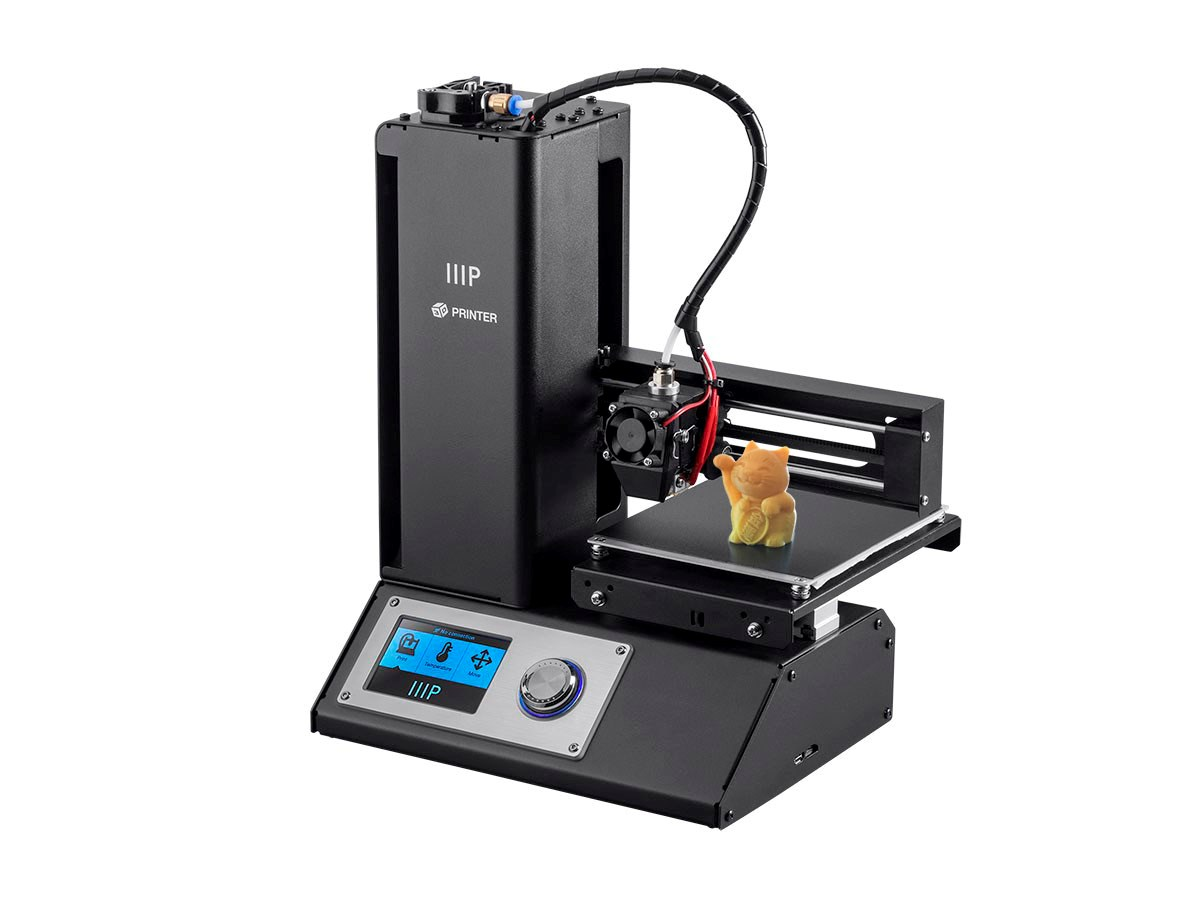
\includegraphics[width=0.5\textwidth]{impresion3.jpg}
	\caption{Impresora FDM: MP Select Mini V2 de Monoprice.}
\end{figure}

\paragraph{SLA (Estereografía)}
Se basa en las propiedades de una resina fotosensible que se solidifica mediante la proyección de un láser (UV) de frecuencia y potencia concreta, ver figura 2.18. (SLA)\cite{impresoras3d-valverde}.

\begin{figure}[H]
	\centering
	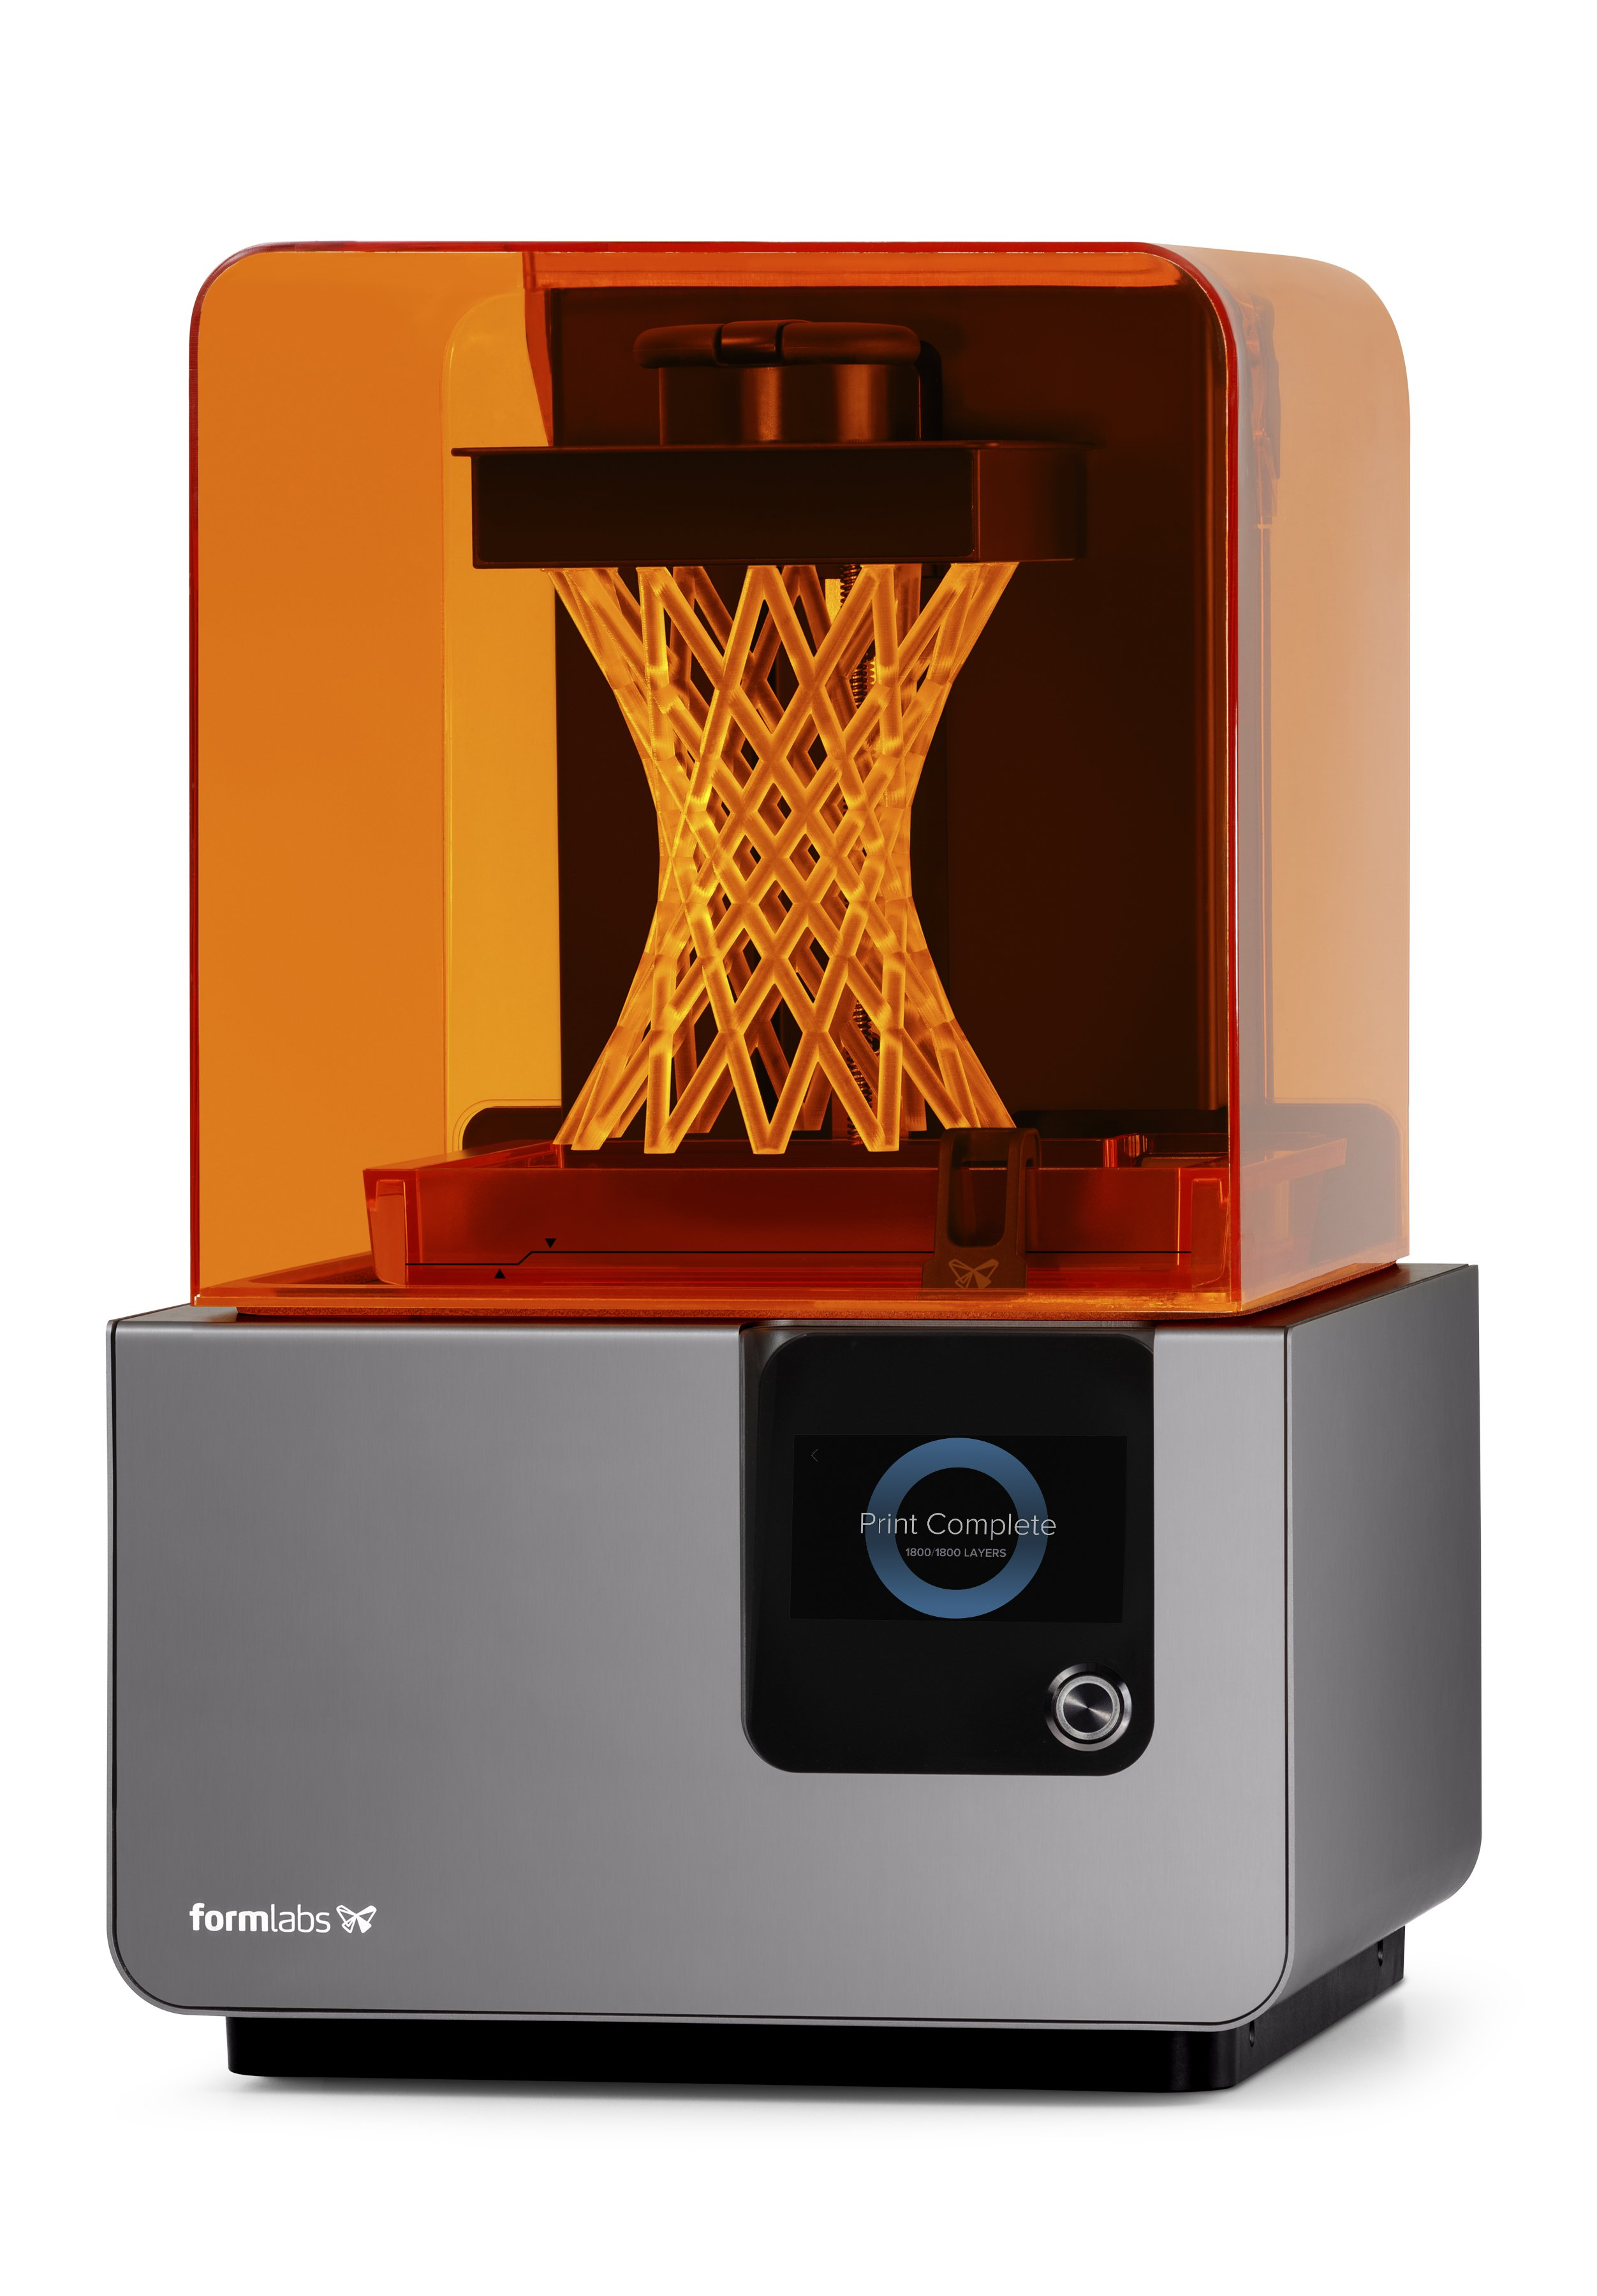
\includegraphics[width=0.3\textwidth]{impresion4.jpg}
	\caption{Impresora SLA: Form2 de Formlabs.}
\end{figure}

\paragraph{DLP (Procesamiento de Luz Digital)}
En este proceso, una cubeta de polímero líquido se expone a la luz de un proyector DLP en condiciones de seguridad. El proyector DLP muestra la imagen del modelo 3D en el polímero líquido, ver figura 2.18 (DLP). El polímero líquido expuesto se endurece y la placa de construcción se mueve hacia abajo y el polímero líquido queda una vez más expuesto a la luz. El proceso se repite hasta que el modelo 3D se completa y la tina se drena de líquido, lo que revela el modelo solidificado\cite{impresoras3d-blog}.

\begin{figure}[H]
	\centering
	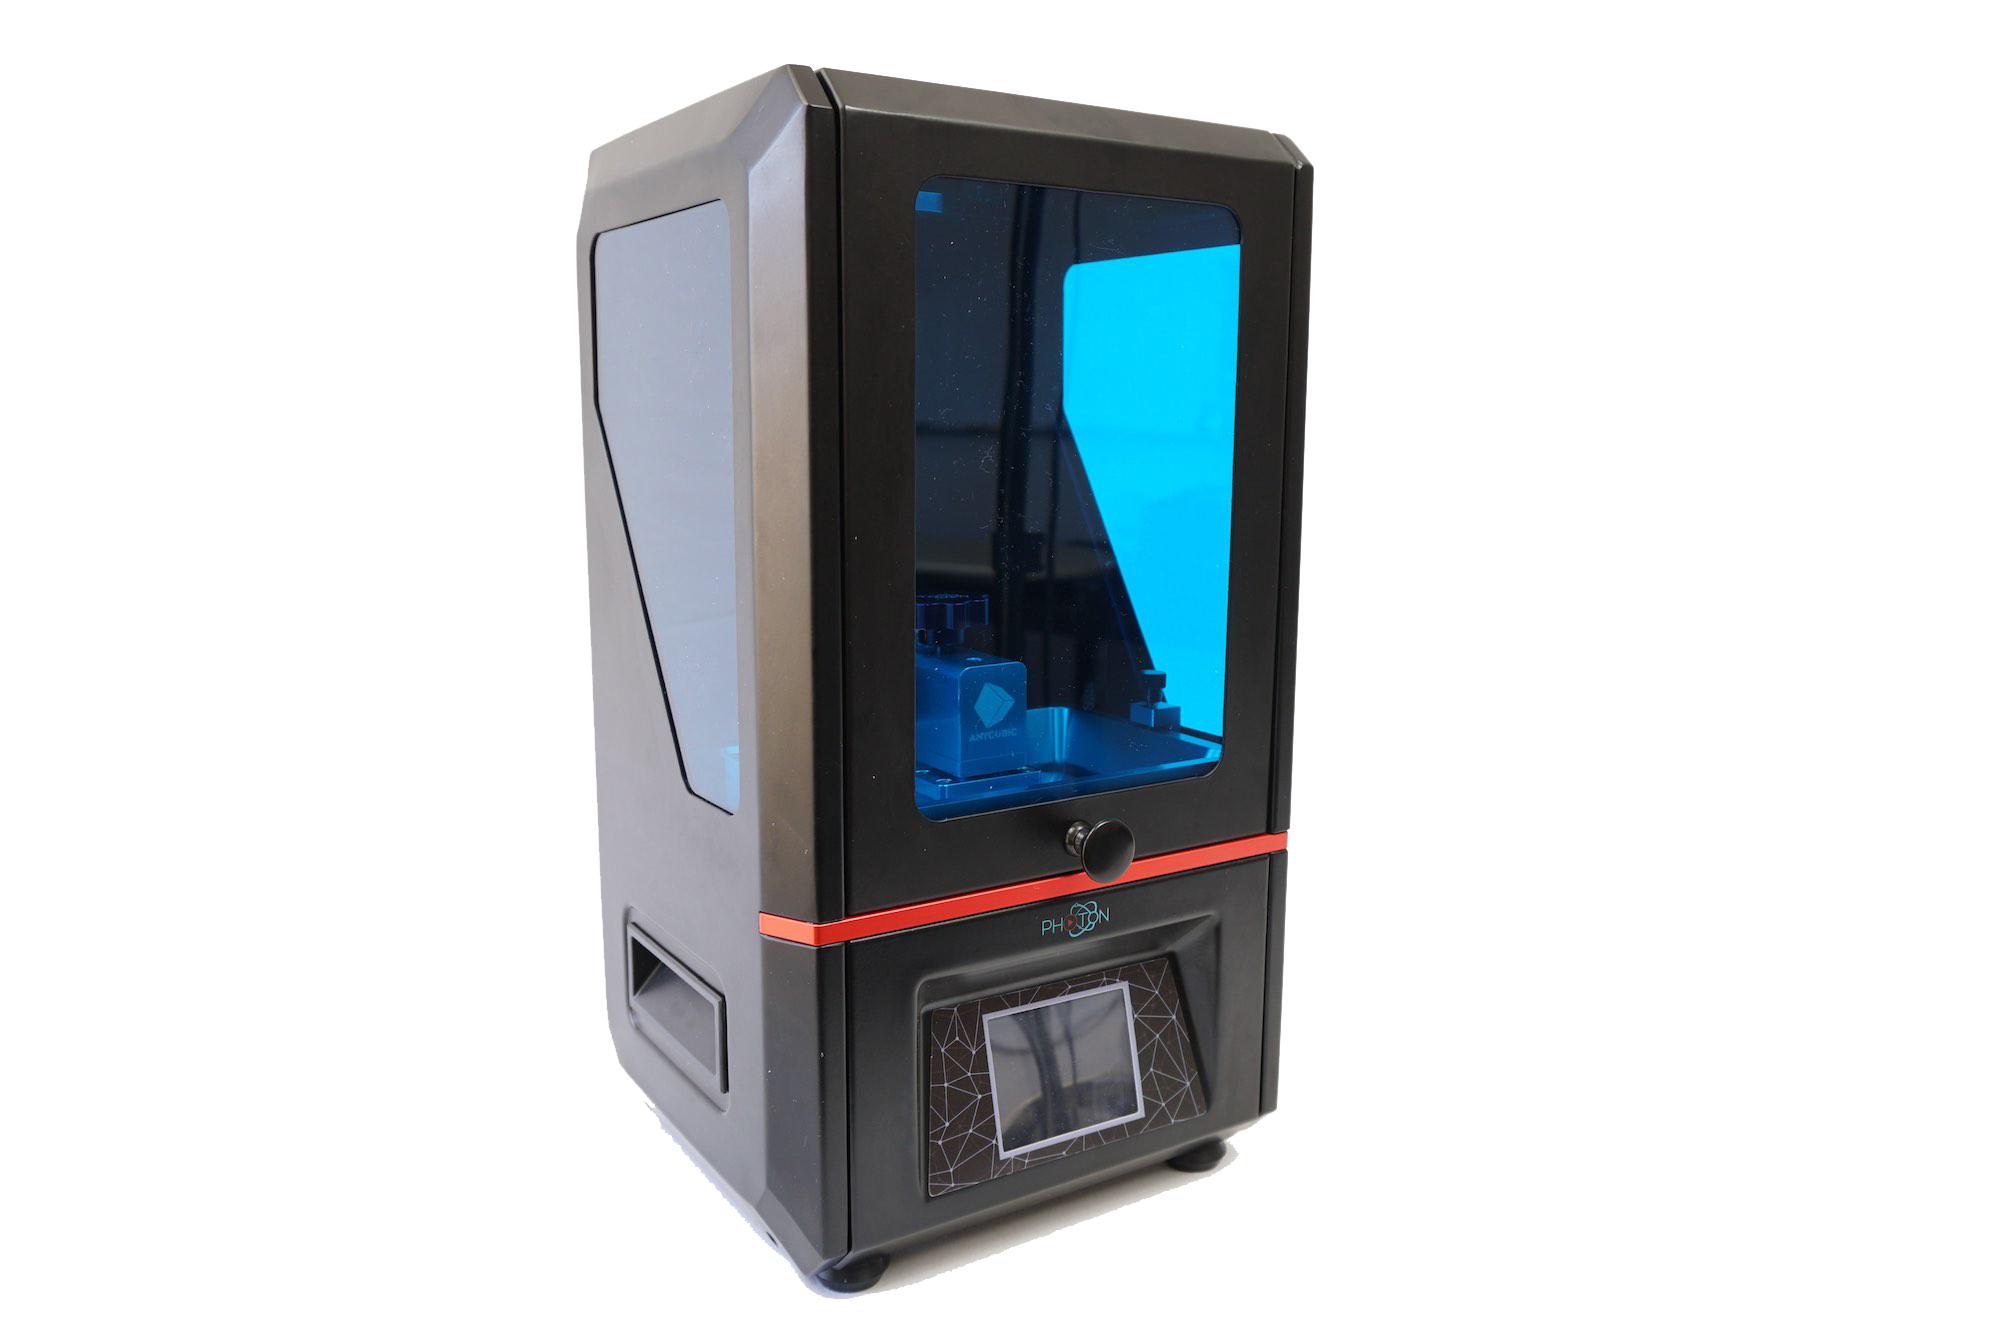
\includegraphics[width=0.5\textwidth]{impresion5.jpg}
	\caption{Impresora DLP: LCD Photon de Anycubic.}
\end{figure}


